% mathematical decoder ring // simulation and nature in design // nervous system & sprout // spring 2010

\documentclass[landscape]{amsart} % Note that if you are producing a
                                  % DVI/PS file, you need to use
                                  % "dvips -t landscape" -- most DVI
                                  % viewers ignore the orientation
                                  % information


%% packages! %%%%%%%%%%%%%%%%%%%%%%%%%%%%%%
\usepackage{graphicx, verbatim, longtable}
% graphicx :: useful for, well, including graphics

% verbatim :: useful for the whole \texttt font and multiline comments

% longtable :: super-convenient package for tables which include
% pagebreaks

\usepackage[cm,empty]{fullpage} % For a 1.5cm border

%% custom configuration %%%%%%%%%%%%%%%%%%%%%%%%%%%%%%

\graphicspath{{diagrams/}} % Where else to look for graphics--this is
                           % expecting a subdirectory called
                           % ./diagrams


%% custom commands! %%%%%%%%%%%%%%%%%%%%%%%%%%%%%%
\providecommand{\norm}[1]{\lVert#1\rVert} % A norm symbol; couldn't
                                          % find a predefined one

\newcommand\Prefix[3]{\vphantom{#3}#1#2#3} % For superscripts on the
                                           % left of a symbol--needed
                                           % for Einstein summation
                                           % notation.  Check out
                                           % http://www.tug.org/pipermail/texhax/2004-February/001650.html
                                           % for details

\renewcommand{\arraystretch}{3} % Changes the cell height spacing,
                                % from
                                % http://chenfuture.wordpress.com/2007/09/20/latex-tabular-more/

\def\imagetop#1{\vtop{\null\hbox{#1}}} % Hack to accomplish vertical
                                       % alignment of images to the
                                       % top of table cells, from
                                       % http://stackoverflow.com/questions/1467351/latex-tabular-vertical-alignment-to-top


%% custom variables! %%%%%%%%%%%%%%%%%%%%%%%%%%%%%%

% each of these is a width of the column containing a . . .
\newlength{\diagramwidth} % diagram
\newlength{\namewidth} % name
\newlength{\notationwidth} % notation
\newlength{\ideawidth} % explanation/idea
\newlength{\usewidth} % use case

\setlength{\namewidth}{1in}
\setlength{\notationwidth}{1in}
\setlength{\diagramwidth}{2in}
\setlength{\ideawidth}{3in}
\setlength{\usewidth}{2in}


% setting the default titles for each column (convenient since each
% field has a separate table)

\def\nametitle{\textbf{the name}}
\def\notationtitle{\textbf{the notation}}
\def\diagramtitle{\textbf{visually}}
\def\explanationtitle{\textbf{the idea}}
\def\usagetitle{\textbf{the use}}

%% conventions %%%%%%%%%%%%%%%%%%%%%%%%%%%%%%
% + diagrams for images are included in a subfolder ./diagrams/ which
% has been named according to the following convention:
% section_name.png, where section and name have -'s wherever spaces
% would be in normal English, e.g. "linear-algebra_transpose.png"
%%%%%%%%%%%%%%%%%%%%%%%%%%%%%%


%%%%%%%%%%%%%%%%%%%%%%%%%%%%%%%%%%%%%%%%%%%%%%%%%% document begins 

\begin{document}

% cover page %%%%%%%%%%%%%%%%%%%%%%%%%%%%%%%%%%%%%%%%%%%%%%%%%%%%%%%%%%%%
\title{a mathematics decoder ring}
\author{simulation and nature in design}
\date{spring 2010}


\maketitle

% TODO: figure out how to fix spacing in Huge

{\Huge This isn't really intended to teach you any math.  It's intended to be the start of a field guide to the notation and ideas convenient for working to make qualitative sense of scientific papers you encounter as you explore techniques and systems you're excited about.

It is a work in progress; if you have any suggestions, errata, or requests, contact \texttt{jesse@n-e-r-v-o-u-s.com}.  Or, if you'd like to volunteer to help to track down good references, make diagrams that don't suck, or volunteer your time as a proofreader, send an email to \texttt{jesse@n-e-r-v-o-u-s.com}.  For more information on the course which it was originally developed for, check out \newline \texttt{http://n-e-r-v-o-u-s.com/education}}

% TODO: figure out how to get URL to wrap nicely


%%%%%%%%%%%%%%%%%%%%%%%%%%%%%%%%%%%%%%%%%%%%%%%%%%%%%%%%%%%%%%%%%%%%%%%%%%%%%%%%
\newpage

\section{vectors}

\begin{longtable}{p{\namewidth}p{\notationwidth}p{\diagramwidth}p{\ideawidth}p{\usewidth}}
\nametitle & \notationtitle & \diagramtitle & \explanationtitle & \usagetitle \\
\hline \\

vector & 
$\boldsymbol{v}$, $\vec{v}$, $V$ &
\imagetop{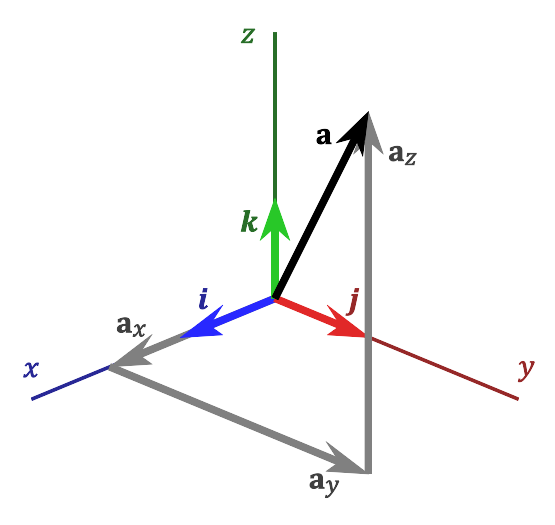
\includegraphics[width=\diagramwidth]{vectors_vector}}   &
Usually, people talk about vectors as representing quantities that have ``both a magnitude and a direction.''  So for example, a force being applied somewhere, in some direction.  Or a speed in a direction (sometimes called a velocity).  Vectors can be a lot more general though, and thinking about them as arrows that you move around and combine in different ways is totally reasonable.  One of the most important things about them is that their size and direction don't change as you switch between coordinate systems. & 
People usually use vectors for indicating positions, forces, and motion.  \\


magnitude, norm, length &
$\norm{\boldsymbol{v}}$ &
\imagetop{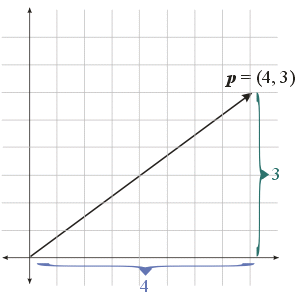
\includegraphics[width=\diagramwidth]{vectors_norm}}   &
This one is pretty simple: it's honestly just the length or size of the vector. &
To talk about the size of whatever they're representing with vectors (\textit{e.g.} speed/velocity, size of force/force) \\


unit vector &
$\hat{u}$, $\boldsymbol{v}$ &
\imagetop{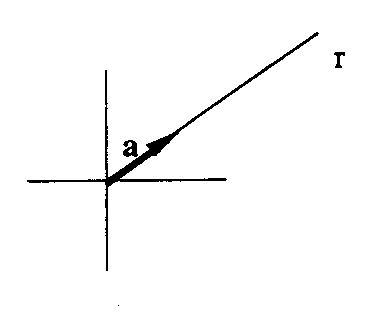
\includegraphics[width=\diagramwidth]{vectors_unit-vector}}  &
It's just a vector of length one.  Usually, you'll see them when people are trying to simplify some calculation. &
Often, it's convenient to be able to get what portion or component of a vector is pointing along a certain direction.  In these cases, if you take the dot product of a vector $\vec{v}$ with a unit vector pointing in some direction, you'll get the portion of $\vec{v}$ which is pointing along the unit vector's direction. \\


basis vectors &
$\hat{i}$, $\boldsymbol{k}$, $e_k$ &
\imagetop{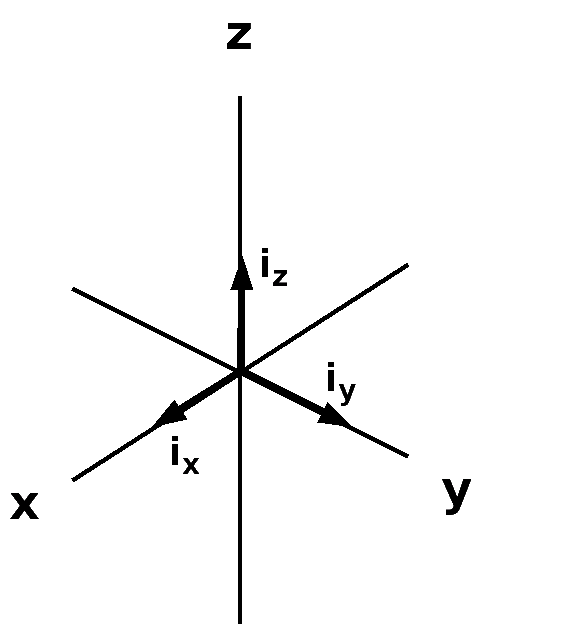
\includegraphics[width=\diagramwidth]{vectors_basis-vectors}} &
A basis is a set of (usually, for convenience, unit) vectors which you can multiply and add together to get any other vector in your space.  So for example, you can multiply and use a combination of unit vectors pointing along the $x-$, $y-$, and $z-$axes to create any other vector in $xyz-$ (\textit{a.k.a} Cartesian) coordinates.   &
Usually, people use basis vectors to represent quantities and equations in a given coordinate system.  Each coordinate (\textit{e.g.} $x$, $y$, and $z$ has a corresponding ``component.''  Sometimes, you'll also see people take the dot product between a basis vector and another vector to find out how much of the other vector is pointing along the basis vector. \\


vector addition &
$\vec{a} + \vec{b}$ &
\imagetop{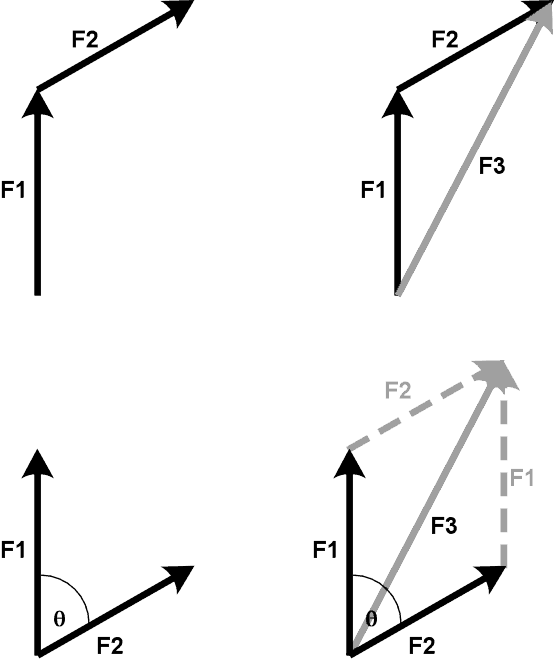
\includegraphics[width=\diagramwidth]{vectors_vector-addition}} &
One way to imagine this is to start at the tail of $\vec{a}$, walk along its length, and then to place $\vec{b}$ at its head (keeping in mind that you can't change the orientation of a vector) and walk along \textit{its} length.  $\vec{a}+\vec{b}$ represents the vector that would connect your starting point ($\vec{a}$'s tail) with your end point ($\vec{b}$'s head). &
Nothing I can think of beyond the obvious. \\


vector subtraction &
$\vec{a} - \vec{b}$ &
\imagetop{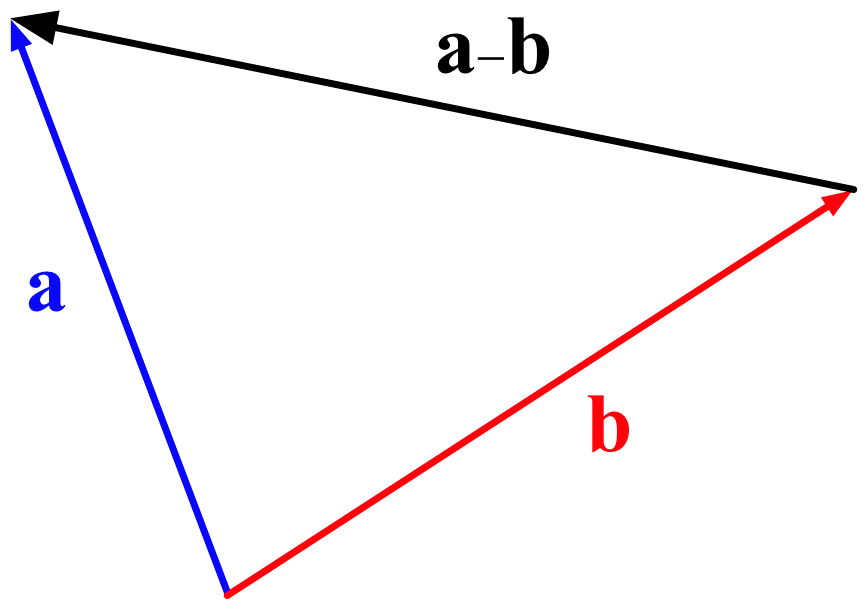
\includegraphics[width=\diagramwidth]{vectors_vector-subtraction}} &
Really, this is the same as $\vec{a} + (-\vec{b})$, where the negative version of a vector ($-\vec{b}$) is simply the same vector, but pointing in the opposite direction. &
Still, nothing I can think of beyond the obvious. \\


scalar multiplication &
$a\vec{v}$, $A\boldsymbol{v}$  &
\imagetop{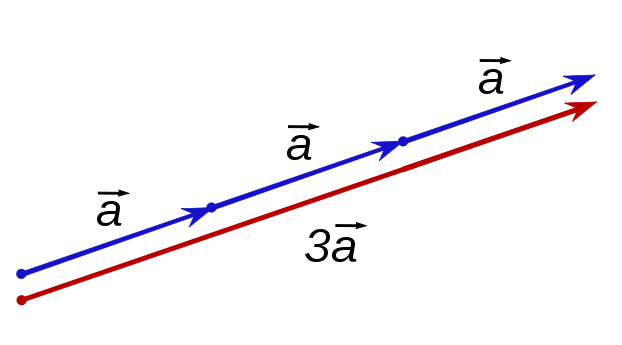
\includegraphics[width=\diagramwidth]{vectors_scalar-multiplication}} &
Multiplying a vector by a scalar can't change the vector's direction, but it can change its length.  So, all $2\vec{a}$ does to $\vec{a}$ is make it twice as long.  Note that you can change the direction of a vector by multiplying it by $-1$. &
Err, scaling the length of vectors? \\


dot product, inner product, scalar product &
$\boldsymbol{a} \cdot \boldsymbol{b}$, $\langle \vec{v}, \vec{u} \rangle$ &
\imagetop{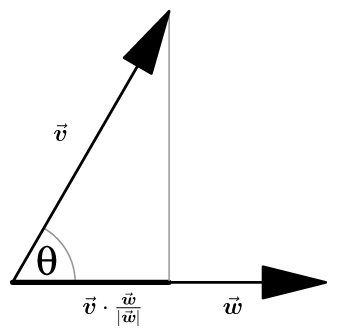
\includegraphics[width=\diagramwidth]{vectors_dot-product}} &
The idea of the dot product is that it can tell you the angle between two vectors.  In some cases, it's easier to think about it as how much one vector ``points along'' another---something often referred to as the ``projection'' of one vector onto another.  &
People usually use the dot product to either project one vector onto another (that is, to describe ``how much'' of one vector is pointing along another) or equivalently, to determine the angle between two vectors (and as a special case, test if two things are perpendicular). \\


cross product, vector product &
$\vec{a} \times \vec{b}$ &
\imagetop{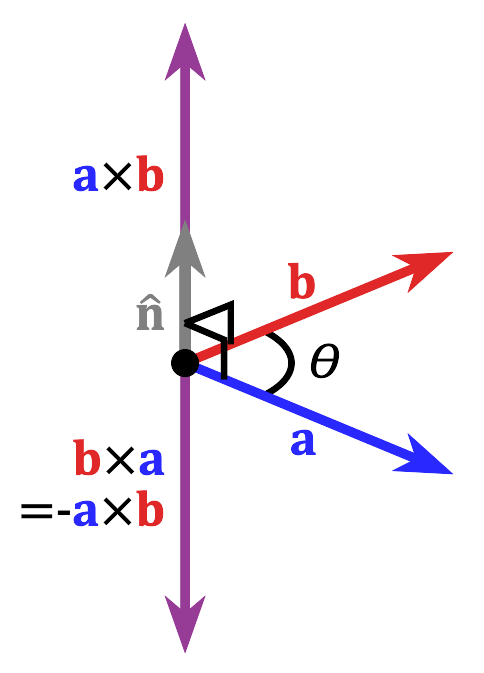
\includegraphics[width=\diagramwidth]{vectors_cross-product}} &
Although it's pretty annoying to compute, the cross product is simple, conceptually: given two vectors, it lets you find a third vector which is perpendicular to the first two. &
People most often use the cross product to find a vector which is perpendicular to two other vectors.  It also figures prominently in the \textit{curl operator}, which lets you measure how much a vector field is curling around a given point. \\


vector field &
$V$, $W$; sometimes, $V:S\rightarrow\mathbb{R}^{n}$ &
\imagetop{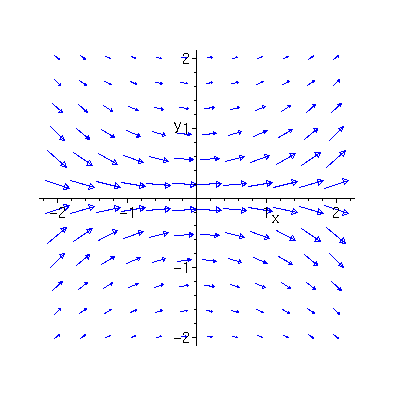
\includegraphics[width=\diagramwidth]{vectors_vector-field}} &
A vector field is a way of associating a vector with every point in space.  You can imagine it as a function which takes in a point in space, and gives you back a vector to put at that point. &
Vector fields are often used for talking about how force fields look in space, and relatedly, how things (especially fluids) flow and move around.  If you've ever seen those smoke visualizations of airplanes in a wind tunnel, that's one way of thinking of a vector field. \\
\end{longtable}

%%%%%%%%%%%%%%%%%%%%%%%%%%%%%%%%%%%%%%%%%%%%%%%%%%%%%%%%%%%%
\newpage

\section{calculus}

\begin{longtable}{p{\namewidth}p{\notationwidth}p{\diagramwidth}p{\ideawidth}p{\usewidth}}
\nametitle & \notationtitle & \diagramtitle & \explanationtitle & \usagetitle \\
\hline \\

derivative, differentiation &
$\frac{dy}{dx}$, $\frac{d}{dx}f(x)$, $\frac{df}{dx}(x)$, $\frac{d^n}{dx}$, $f\prime$, $f^{(n)}$, $\dot{f}$, $\ddot{f}$, $D_xf(x)$, $D_xy$, &
\imagetop{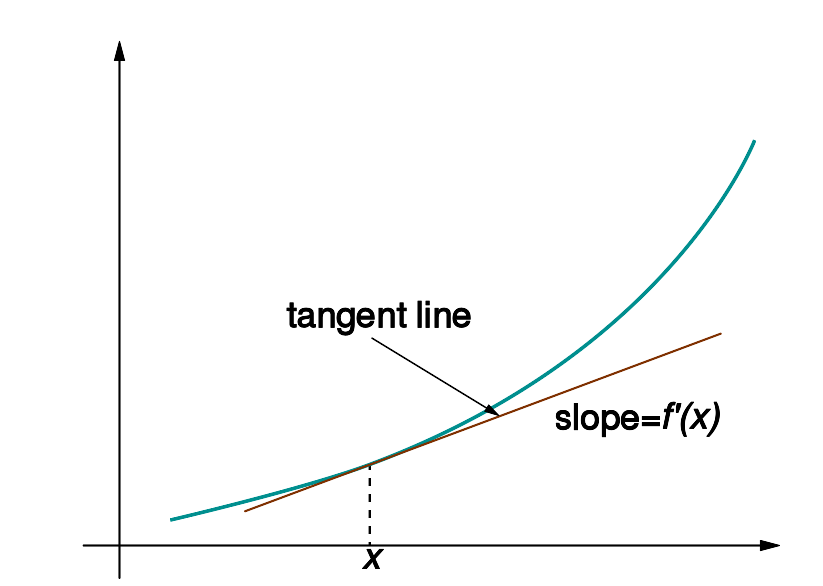
\includegraphics[width=\diagramwidth]{calculus_derivative}} &
At its most basic, a derivative measures how quickly something is changing at a given point.  For a function, this is the same as talking about the ``slope of the tangent line''---that just means that when a function is changing quickly, it has a lot steeper slope, and when it changes slowly, that it's a lot flatter. &
Derivatives and differentiation show up everywhere.  People use derivatives to describe how different rates of change relate to one another, to find the maximum and minimum of functions, to do all sorts of neat stuff. \\


integral, integration, antiderivative &
$\int_S f dx$, $\int_a^b f dx$, $\iiint_V f dx dy dz$  &
\imagetop{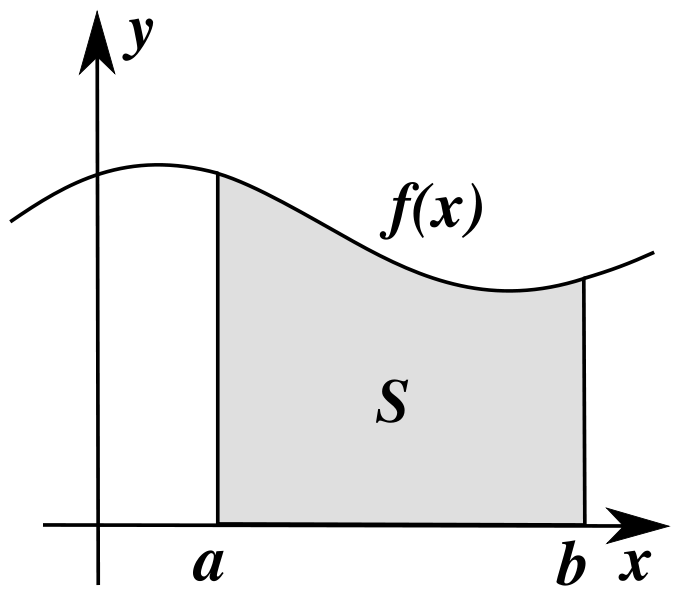
\includegraphics[width=\diagramwidth]{calculus_integral}} &
Conceptually, integrals are pretty simple: they tell you how much area (or volume) is enclosed by a function (or a surface).  That's why you hear people talking about ``area under the curve'' all the time.  Amazingly, it also turns out that integrals are kinda like the opposite of derivatives: the integral of a derivative of a function is that same function (and vice versa).  &
People use integrals to do all sorts of things: some of the most common include finding the area/volume of a curve/surface and solving equations that have derivatives in them. \\


partial derivative, directional derivative &
$D_{\vec{v}}$, $D_{\boldsymbol{v}}$, $\frac{\partial u}{\partial x}$, $f_{xy}$, $\partial_xf$, $f^{\prime}_{x}$  &
\imagetop{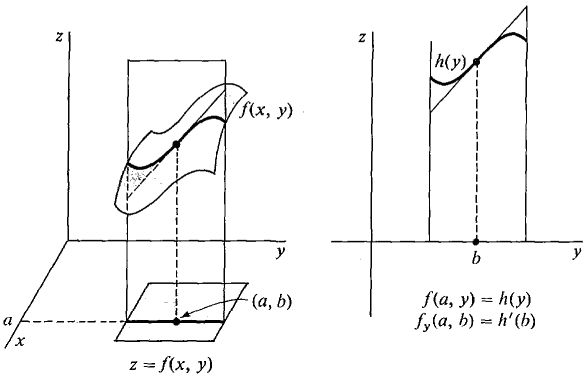
\includegraphics[width=\diagramwidth]{calculus_partial-derivative}} &
A partial derivative is pretty simple: when people normally talk about derivatives, they're talking about the change in one thing respect to another (position with respect to time, $y$ with respect to $x$, whatever.  If you have many variables---all of which can change---a partial derivative lets you answer the question, ``When I hold $v_3$ constant, how much does $v_1$ vary?'' Another way of thinking about it is: when you move perpendicular to one axis, how much does the function's value on the other axis change?&
Partial derivatives are used to describe how different rates of change relate to one another.  Often, you will have a system where there are several different relationships between a handful of rates of change, but whose relationship can only be described when you keep everything else constant.  (For example, the radius, height, and volume of a cone are interrelated, but you can only talk about the changes in rates of change if you can say, ``Well, keeping the height constant, the rate of change of the radius and volume are related as \ldots'' \\


divergence, div &
$\nabla \cdot \boldsymbol{v}$, div $\boldsymbol{v}$  &
\imagetop{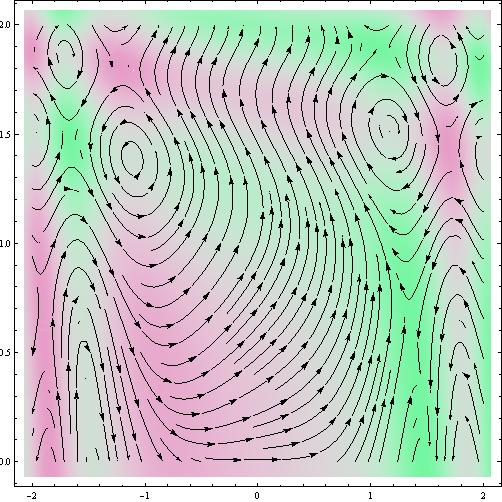
\includegraphics[width=\diagramwidth]{calculus_divergence}} &
The divergence is a way of talking about how much a vector field points into or out of a given point.  Another way people say this is by describing it as ``How much is the vector field acting as a source or a sink at a given point?''  &
For a handful of interesting reasons, the divergence comes up in a lot of mathematical descriptions of physical laws---for example, it features prominently in Maxwell's equations (the laws which govern how electric and magnetic fields behave). \\


gradient, grad &
$\nabla f$, grad $f$ &
\imagetop{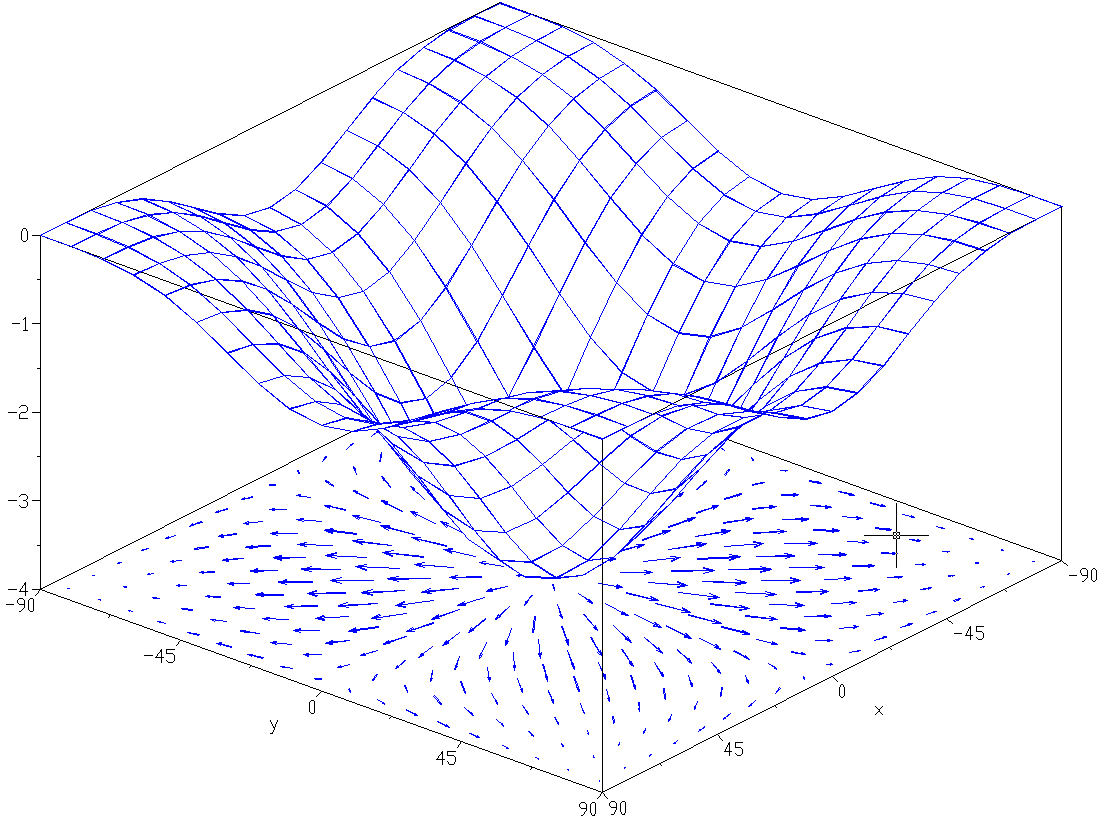
\includegraphics[width=\diagramwidth]{calculus_gradient}} &
The gradient takes a function (it's usually has $\geq 3$ dimensions) and gives you a vector field which tells you---at every point---what direction the greatest increase is in, and what the size of that increase is.  So if you imagine a function that tells you the height of a hill at every point, the gradient at each point would point in the direction of steepest ascent. &
The gradient is another tool that shows up all the time in describing physical laws (especially in fluid dynamics and thermodynamics). \\


curl, rotor, rotational &
$\nabla \times \boldsymbol{v}$, curl $\boldsymbol{v}$, rot $\boldsymbol{v}$ &
\imagetop{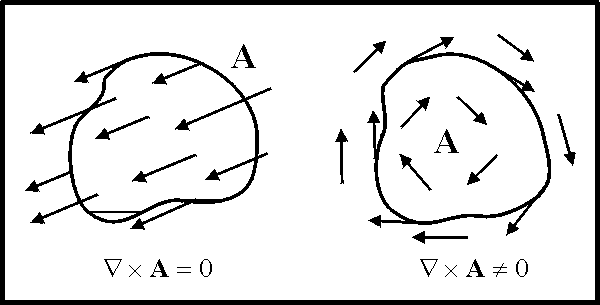
\includegraphics[width=\diagramwidth]{calculus_curl}} &
The curl operator tells you how much a given vector field is rotating (or curling) around a certain point.  You can kinda think of it as the extent to which a vector field is whirlpooling around a point.  If you imagine your vector field as the flow of water, the curl tells you how much (and in what direction) a little boat would spin if you were to place it at a given point. &
The curl shows up a lot in discussions of fluid flow, and is another one of those operators that you end up talking about a surprising amount when you're writing down physical laws (again, especially those which deal with fluids or fluid-like things. \\


Laplacian, Laplace operator &
$\delta f$, $\nabla^2 f$, $\nabla \cdot \nabla f$  &
\imagetop{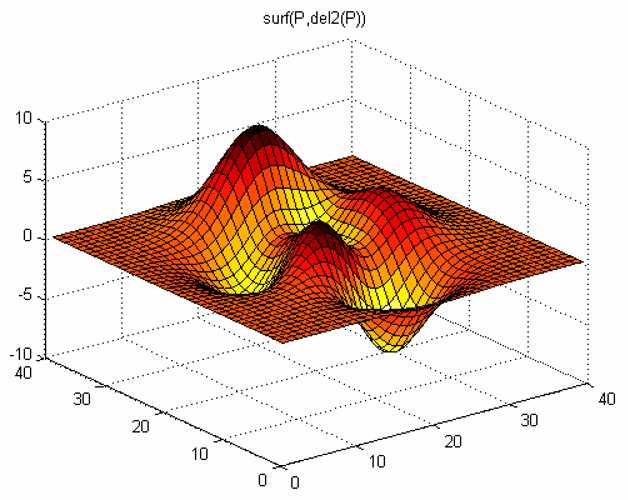
\includegraphics[width=\diagramwidth]{calculus_laplacian}} &
Intuitively, the Laplacian tells you how much the value of something at a given point differs from the average value of the values at that points' neighbors.  So if we're talking about a function $F$, that means that the Laplacian tells you how much $F(p_0)$ differs from the average of $F$ at all the points around $p_0$.  Another way of saying this is that the Laplacian tells you how much curvature or curviness there is at every point in a surface or function. &
The Laplacian shows up a lot in talking about systems which are very efficient (that is, they do not dissipate a lot of energy---they are roughly conservative).  This includes everything from talking about electrostatics to heat flow. \\
\end{longtable}

%%%%%%%%%%%%%%%%%%%%%%%%%%%%%%%%%%%%%%%%%%%%%%%%%%%%%%%%%%%%
\newpage

\section{linear algebra} 

\begin{longtable}{p{\namewidth}p{\notationwidth}p{\diagramwidth}p{\ideawidth}p{\usewidth}}
\nametitle & \notationtitle & \diagramtitle & \explanationtitle & \usagetitle \\
\hline \\

matrix &
$A$, $B$, $M$ &
\imagetop{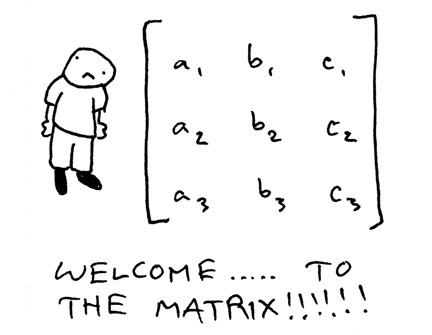
\includegraphics[width=\diagramwidth]{linear-algebra_matrix}} &
Really, a matrix is just a way of holding a bunch of numbers or other pieces of information and organizing them so that you can do some other types of math with them. &
Pretty much every topic has some way of representing or discussing it in such a way that it involves a matrix or uses linear algebra ideas. \\


transpose &
$A^{T}$, $A\prime$, $A^{\mbox{tr}}$, $\Prefix^{A}{t}$ &
\imagetop{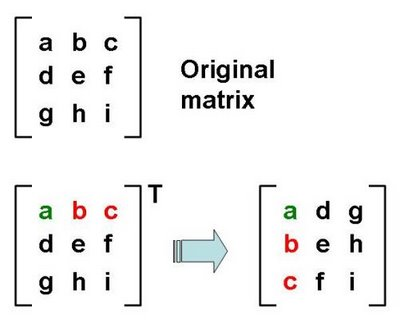
\includegraphics[width=\diagramwidth]{linear-algebra_transpose}} &
The transpose of a matrix is just the matrix you'd get if you took each row and turned it into a column (so the first row becomes the first column of the transpose, the second row the second column, and so on). &
It shows up in a lot of matrix math because it turns out to have some convenient mathematical properties, but I don't think there are especially common uses. \\


Einstein [summation] notation &
$c_ix^i$ &
not that I can think of &
This is kinda annoying, but especially in physics and linear algebra, you'll see people use this as shorthand to represent a sum over all possible values of an index variable.  An index variable is just a variable you use to keep track of the components of some collection.  For example, people often write the $n$th element of a vector $\vec{v}$ as $\boldsymbol{v}_n$.  According to Einstein notation, when an index variable appears twice in a single term, once in an upper (superscript) and once in a lower (subscript) position, it implies a sum over all the possible values of the index variable. &
For making summations more convenient to write and (for some people) easier to read.  You don't really see this outside of physics and linear algebra, though.\\


inverse &
$A^{-1}$ &
uhh$\ldots$ &
The inverse (let's call it $B$) of a matrix $A$ is a matrix such that $AB = I$.  Keep in mind that $I$ is the closest thing linear algebra has to the number one, so in some ways, you can think of the inverse of a matrix as kind of like dividing by that matrix.  Or, if you're thinking about the effect a matrix has something, the inverse of that matrix undoes that effect (for instance, if multiplying by one matrix rotates a shape, multiplying by its inverse will un-rotate it).  &
People use inverses for all sorts of things---the most common use is to undo the operation of a matrix. \\


identity matrix &
$I_1$, $I_2$, $I_n$ &
\imagetop{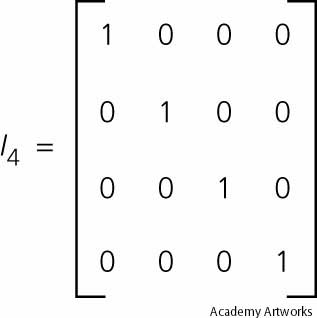
\includegraphics[width=\diagramwidth]{linear-algebra_identity-matrix}} &
The identity matrix is the closest thing linear algebra has to the number on. &
I'm not sure there is a most common use for it---it really does often function like the number one. \\


determinant &
det $A$, $\left| A \right|$ &
\imagetop{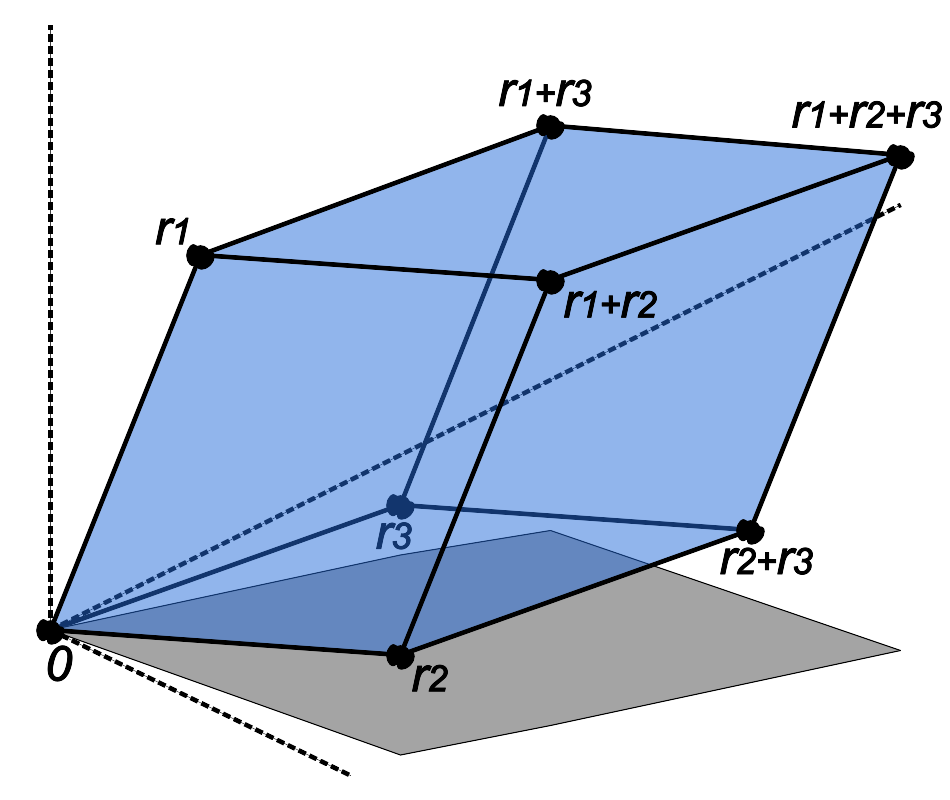
\includegraphics[width=\diagramwidth]{linear-algebra_determinant}} &
The most geometric understanding of the determinant is as a scale factor: if a matrix has a determinant of two, that means that when that matrix is applied to a set of points, it will double that set of points' area. &
Three of the most common uses for the determinant are using it to find out whether a matrix is invertible, to calculate volume, and to scale different shapes (stretching them to make them bigger or smaller). \\


eigenvector &
nothing unusual---just like normal vectors &
\imagetop{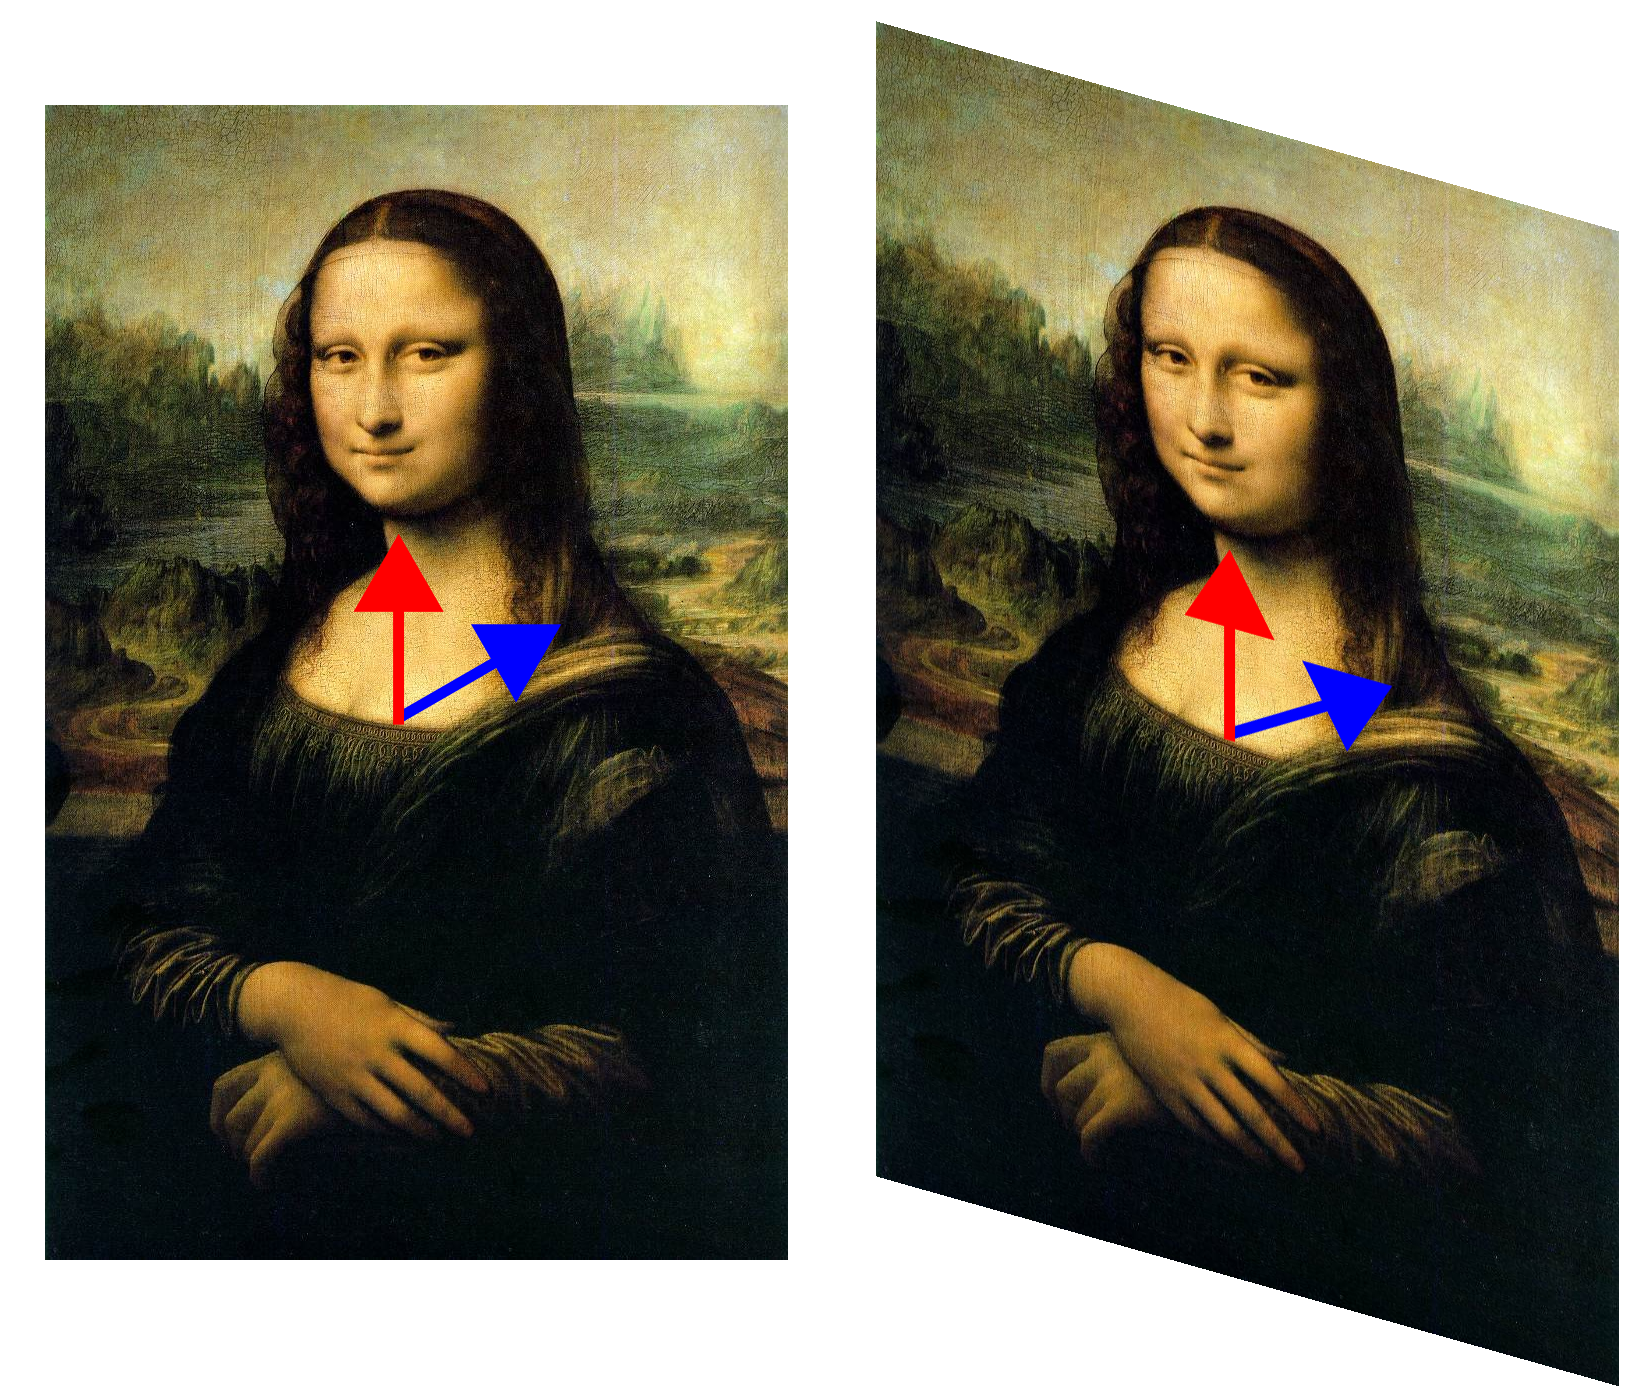
\includegraphics[width=\diagramwidth]{linear-algebra_eigenvector}} &
If you think about matrices as representing transformations that you can apply to vectors, the eigenvectors of a given matrix are those which would not be rotated (though they may be scaled) after the application of that matrix. &
Eigenvectors are especially useful in factoring matrices (that is, writing a matrix $M$ as the product of other matrices). \\


eigenvalue &
$\lambda_i$ &
\imagetop{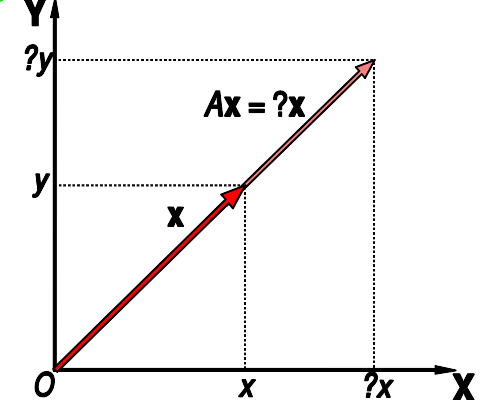
\includegraphics[width=\diagramwidth]{linear-algebra_eigenvalue}} &
If you think about matrices as representing transformations that you can apply to vectors, the eigenvalues of a given matrix are the scale factors by which that matrix scales its eigenvectors. &
It turns out these are really useful in factoring matrices, too. \\
\end{longtable}

%%%%%%%%%%%%%%%%%%%%%%%%%%%%%%%%%%%%%%%%%%%%%%%%%%%%%%%%%%%%
\newpage


%%%%%%%%%%%%%%%%%%%%%%%%%%%%%%%%%%%%%%%%%%%%%%%%%%%%%%%%%%%%
% END OF TYPESET TEXT
%%%%%%%%%%%%%%%%%%%%%%%%%%%%%%%%%%%%%%%%%%%%%%%%%%%%%%%%%%%%
\begin{comment}
Here's a template for tables for a domain:

\begin{longtable}{p{\namewidth}p{\notationwidth}p{\diagramwidth}p{\ideawidth}p{\usewidth}}
\nametitle & \notationtitle & \diagramtitle & \explanationtitle & \usagetitle \\
\hline \\


NAME &
NOTATION &
\imagetop{\includegraphics[width=\diagramwidth]{section_diagram}} &
IDEA &
USE \\

\hline \\


\end{longtable}

\end{comment}


\end{document}